\section{Our model and approach}
\label{sec:approach}
We now develop our model and use it to specify our problem more
precisely. We then present our algorithm to address our ailment
prediction problem.

\subsection{General-purpose topic modeling over time with \tmlda}
To take into account the evolution of the underlying topics of a
dynamic collection of documents with time (e.g., a microblog or a
facebook page) Wang et al. (2012) introduced a modified version of the
LDA model, \tmlda~\cite{DBLP:conf/kdd/WangAB12}.
In ~\cite{DBLP:conf/kdd/WangAB12}, \tmlda was introduced to extend
lda with modeling topic evolution of dynamic collection of documents over time
 Topic distribution
of the $i$--th document, $\theta_i$  is ascertained from 
the topic distribution of the previous document, $\theta_{i-1}$.
At the heart of the algorithm lies the following equation.
\begin{equation}
	\label{eq:tmlda:basic}
	\theta_{i}\approx\frac{\theta_{i-1}.M}{\|\theta_{i-1}.M\|_{\ell_1}}
\end{equation}
where $M$ is a $k\times k$ matrix, called the transition
matrix, and $k$ is the number of topics. To obtain the transition matrix, 
the authors propose to solve the following least square
problem ($\|\cdot\|_F$ denotes the Frobenius norm and X denotes the search space):
\begin{equation}
	\label{eq:tmlda:train}
	M=\argmin_X{\|A.X-B\|_F}
\end{equation}
where $A$ and $B$ are as specified below.
\begin{equation}
	\label{eq:tmlda:vectors}
	A=\begin{pmatrix}\theta_{1}\\\vdots\\\theta_{i-1}\end{pmatrix},\,B=\begin{pmatrix}\theta_{2}\\\vdots\\\theta_{i}\end{pmatrix}
\end{equation}
However, while being quite elegant in modeling general purpose topics
\tmlda is not specialized to capture \texttt{\emph{health}} transitions
over time.
\subsection{\tmatam: Modeling Health Topics over Time}
\label{subsec:model}
While \atam is effective at modeling health-related topics, 
it is not designed to model topic transitions over time. 
We hence propose \tmatam that builds on top of \atam and \tmlda. 
\tmatam computes the aggregate topic distribution, $\Theta_g^t$, 
of a set of documents $D_g^t$. Qualitatively, the topic distribution 
has the following components. 
\begin{itemize}
\item $\eta_g^t$ : Distribution over ailments in $D_g^t$
\item $\theta_g^t$ : Distribution over general topics in $D_g^t$
\item $\Theta_g^t=\begin{pmatrix}(1-\pi)\theta_g^t& \pi\eta_g^t\end{pmatrix}$ 
where $\pi$ is the proportion of non-health words related to some 
aspect of an ailment. We show $\Theta$ for an example tweet in 
Figure~\ref{fig:exampleTweet2}.
\end{itemize}
\begin{figure}[b!]
\centering
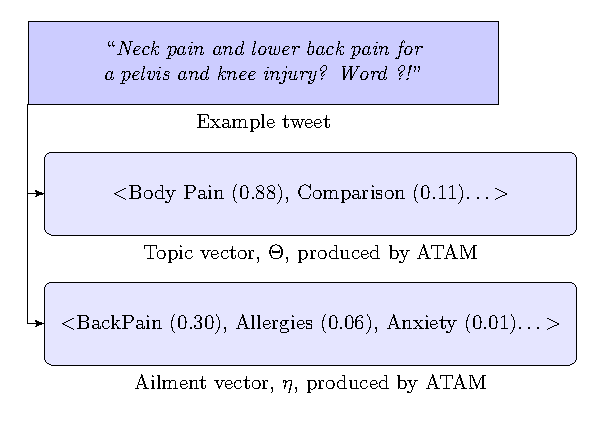
\includegraphics[width=0.45\textwidth]{tikz/exampleTweet2.pdf}
\caption{$\Theta$ predicted by \atam on an example tweet, while $\eta$ predicted by ATAM on region containing example tweet}
\label{fig:exampleTweet2}
\end{figure}

\tmatam, at its heart, solves following equation.
\begin{equation}
A_g^{t}\approx A_g^{t-1}.M
\end{equation}
where
\begin{equation}
A_g^{t-1}=\begin{pmatrix}\Theta_g^1\\\vdots\\\Theta_g^t\end{pmatrix},\,A_g^t=\begin{pmatrix}\Theta_g^2\\\vdots\\\Theta_g^{t+1}\end{pmatrix}%d_g^{t-1}=\begin{pmatrix}P_1\\\vdots\\P_t\end{pmatrix},\,d_g^t=\begin{pmatrix}P_2\\\vdots\\P_{t+1}\end{pmatrix}
\end{equation}
$M$ is an unknown transition matrix which is obtained by solving the following least square problem.
\[
\min_M\|A_g^t- A_g^{t-1}.M\|_F
\]
\tmatam thus learns a transition matrix which is used to model health topics.

\subsection{Ailment prediction problem revisited}
\label{subsec:problem}
We are now ready to revisit our problem: Given a set of
documents $D_g^{t_{i-1}}$ formed by tweets originating from a region
$g \in G$ during time period $t_{i-1}$, predict $\eta_g^{t_i}$, the
ailment distribution of documents in $D_g^{t_i}$, corresponding to
posts from $g$ in period $t_i$ from $\Theta_g^{t_{i-1}}$, the ailment
distribution of document $D_g^{t_{i-1}}$ corresponding to posts from
$g$ during period $t_{i-1}$.  Our framework can predict $\eta_g^{t_i}$, $\theta_g^{t_i}$ or $\Theta_g^{t_i}$
 but in our experiments, we found  using $\Theta_g^{t_{i-1}}$ to predict $\eta_g^{t_i}$ is the most interesting to our cause.  

\subsection{Algorithm}
\label{subsec:tmalg}
Algorithm~\ref{alg:tmatam} contains the steps of our solution. It has 
two main parts: {\texttt{\emph{ \change detection}}} and {\texttt{\emph{ ailment prediction}}}. 
We first describe how \changes are detected then we show how ailment topics being discussed in twitter 
are predicted over time within \seasons.

\paragraph{\change Detection}
We use $\mf Z$ to refer to the set of all health-related and non-health 
related topics. For each region $g \in \mf G$ (Line~\ref{alg:line:start}) 
we first run \atam over the full time period $D_g$ (Line~\ref{alg:line:atam}).
Next for each period $t\in \mf T$ (Line~\ref{alg:line:tstart}), 
we use the output of \atam over $D_g$ to generate 
topic distribution $\Theta_g^t$ (Lines~\ref{alg:line:createThetaStart}--
\ref{alg:line:createThetaEnd}). 
Note that, $\Theta_g^t$ includes general-purpose topics as well as ailments that are
discussed in tweets originating from region $g$ during time period $t$.  
% \comment{
% \begin{figure}[b!]
% \centering
% \includegraphics[width=0.45\textwidth]{tikz/Thetaatam.pdf}
% \caption{$\Theta_{atam}$ - Topic distribution vector as predicted by ATAM on a tweet}
% \label{fig:atamTheta}
% \end{figure}
% \begin{figure}[b!]
% \centering
% \includegraphics[width=0.45\textwidth]{tikz/ThetaatamContrast.pdf}
% \caption{$\Theta_{atam}$ - Topic distribution vector as predicted by ATAM on a second tweet}
% \label{fig:atamTheta2}
% \end{figure}
% } 
Next we examine the distance between consecutive distributions
$\Theta_g^{t-1}$ and $\Theta_g^t$ of the region $g$ 
to identify the most significant \texttt{\emph{\change}}, $t_c$ (Line~\ref{alg:line:ThetaDiff}).
We treat the choice of distance measure $m$ as black box, 
which could be \emph{Bhattacharya Distance}\footnote{\url{https://en.wikipedia.org/wiki/Bhattacharyya_distance}} or \emph{Cosine Similarity}\footnote{\url{ https://en.wikipedia.org/wiki/Cosine_similarity}}. 
The time period $t_c$ is termed as the \texttt{\emph{\change}} for
region $g$. The entire span of time, $[t_1\ t_{|\mf T|}]$, is divided 
into two intervals, \emph{pre}, consisting
of all time periods prior to the \emph{\change} (Line~\ref{alg:line:buildSeasonPre}), 
and \emph{post}, consisting of all time periods after 
the \emph{\change} (Line~\ref{alg:line:buildSeasonPost}).

We term these intervals as \seasons w.r.t ailments being discussed in twitter. Qualitatively, \season is a 
time interval (collection of consecutive time periods) during which
the tweets originating from the region are homogeneous in terms of ailment topics. 
The \texttt{\emph{\change}} characterizes a significant change point
in the evolution of ailments. We posit that such change points exist. These change points in ailment topic discussions
may be caused by onset of the disease or some other external factors. Nevertheless, they are the interesting points for analyzing purposes.
Such analysis may lead to various insights into onset of diseases.
Onset of disease is usually affected by several factors, such as weather, which may cause
a sudden onslaught of ailments different from the ones that were in circulation
previously. The pervasive nature of communicable diseases is also a contributing
factor. Note that the results in Figure~\ref{fig:ailmentsEvolve} support our assumption.

\paragraph{Ailment Prediction}
The key idea in \tmatam is to identify \emph{\changes} and predict
evolution of topics within each \season. This is a fresh departure
from existing solutions that operate in a \season-agnostic fashion.
By definition, a \season is (nearly) homogeneous in terms
of ailments. In other words, the ailments evolve in a smooth fashion
within a \change and change abruptly across \change boundaries.
In this study, we limit ourselves to finding a single \change boundary for
each region $g$. While this may not be true for all regions, we obtain
significant improvement in terms of prediction accuracy over the previous
state of the art with just a single boundary.
We outline in lines~\ref{alg:line:predStart}--\ref{alg:line:predEnd} 
of Algorithm~\ref{alg:tmatam} the steps undertaken. 
\begin{algorithm}[t]
\caption{TM-ATAM: \change Detection and Training Ailment Distribution Predictor}
\label{alg:tmatam}
\begin{algorithmic}[1]
 \ForAll {$g \in G$}\label{alg:line:start}
 \State Run ATAM on $D_g$\label{alg:line:atam}
 \ForAll  {$t \in \mf T$}:\label{alg:line:tstart}
 \ForAll {$z \in \mf Z$}:\label{alg:line:createThetaStart}
 \State $\Theta_g^t[z] \leftarrow 0$
 \EndFor
 \ForAll {$d \in D_g^t$}:
 \ForAll {$w \in d$}:
 \State $z \gets topic(w)$
 \State $\Theta_g^t[z] \gets \Theta_g^t[z] + \frac{1}{|d|\times |D_g^t|}$
 \EndFor
 \EndFor\label{alg:line:createThetaEnd}
 \EndFor
 \State $\displaystyle t_{c} = \argmax_t{\ m(\Theta_g^{t-1},\ \Theta_g^{t})}$\label{alg:line:ThetaDiff}
 \State $pre = [t_1\ ,\ t_{c-1}]$\label{alg:line:buildSeasonPre} 
 \State $post = [t_{c}\ , \ t_{|\mf T|}]$\label{alg:line:buildSeasonPost} 
 \ForAll {$s \in \{pre,\ post\}$}:\label{alg:line:predStart}
 \State $A_g^t\approx A_g^{t-1}.M$
 \State $M =(A_g^{t-1\intercal}A_g^{t-1})^{-1}A_g^{t-1\intercal}A_g^t$
 %\State $M = A_g^{t-1}\textsuperscript{\textdagger}A_g^t=(A_g^{t-1\intercal}A_g^{t-1})^{-1}A_g^{t-1\intercal}A_g^t$
 \EndFor\label{alg:line:predEnd}
\EndFor\label{alg:line:end}
\end{algorithmic}
\end{algorithm}

\subsection{Time-Aware Ailment Topic Aspect Model (T-ATAM)}

\begin{figure}[ht]
  \begin{center}
    \documentclass[a4paper]{article}

\usepackage{tikz}
\usetikzlibrary{bayesnet}
\title{Time-Aware Ailment Topic Aspect Model}
% \author{Sumit Sidana}

\begin{document}

\maketitle

  % Define nodes
  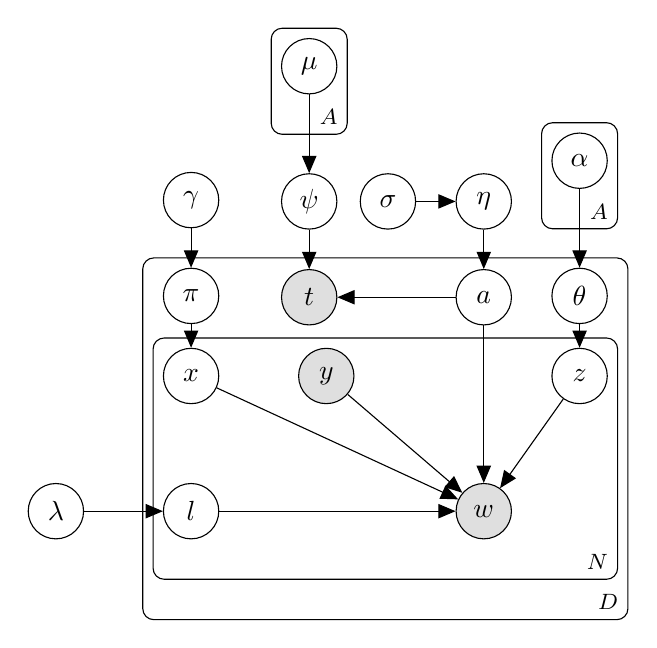
\begin{tikzpicture}[x=1.7cm,y=4.8cm]
  % Nodes

  \node[obs]                   (word)      {$w$} ; %
  \node[latent, left=3cm of word] (background) {$l$};
  \node[latent, above=1cm of background] (route) {$x$};
  \node[obs, right=1cm of route]    (aspect)      {$y$} ; %
  \node[latent, right=2.5cm of aspect]    (topic)  {$z$}; %
  \node[latent, above=2cm of word] (ailment) {$a$};
  \node[obs, left=1.5cm of ailment] (timestamp) {$t$};
  \node[latent,above=0.3cm of topic] (theta){$\theta$};
  \node[latent,above=0.3cm of route] (pi){$\pi$};
  \node[latent,left=1cm of background](lambda){$\lambda$};
  \node[latent,above=0.5cm of ailment](eta){$\eta$};
  \node[latent,left=0.5cm of eta](sigma){$\sigma$};
  \node[latent,above=0.5cm of pi](gamma){$\gamma$};
  \node[latent,above=0.5cm of timestamp](psi){$\psi$};
  \node[latent,above=1cm of psi](mu){$\mu$};
  \node[latent,above=1cm of theta](alpha){$\alpha$};
 
%   \node[const, above=of topic] (atheta) {$\alpha_\theta$};
  
\edge {background,route,aspect,topic,ailment} {word} ;
\edge {ailment}{timestamp}
\edge {theta}{topic}
\edge {pi}{route}
\edge {lambda}{background}
\edge {eta}{ailment}
\edge {sigma}{eta}
\edge {gamma}{pi}
\edge {psi}{timestamp}
\edge {mu}{psi}
\edge {alpha}{theta}

  \plate {plate1} {(word)(background)(route)(aspect)(topic)} {$N$} ;
  \plate {} {(word)(background)(route)(aspect)(topic)(ailment)(timestamp)(theta)(pi)(plate1)}{$D$};
  \plate {} {(mu)}{$A$}
  \plate {} {(alpha)}{$A$}
  % Factors
%   \factor[above=of X]     {X-f}     {Multi} {} {} ; %
%   \factor[above=of T]     {T-f}     {left:Multi} {} {} ; %
%   \factor[above=of theta] {theta-f} {left:Dir} {} {} ; %

  % More nodes
%   \node[latent, right=of X-f] (phi)  {$\phi$}; %
%   \node[const, above=of phi]  (aphi) {$\alpha_\phi$}; %

%   \factor[above=of phi] {phi-f} {right:Dir} {} {} ; %

%   \factoredge {theta}  {T-f}     {T} ; %
%   \factoredge {atheta} {theta-f} {theta} ; %
%   \factoredge {phi}    {X-f}     {X} ; %
%   \factoredge {aphi}   {phi-f}   {phi} ; %
% 
%   \gate {X-gate} {(X-f)(X-f-caption)} {T}

%   \plate {plate1} { %
%     (X)(X-gate) %
%     (T)(T-f)(T-f-caption) %
%   } {$\forall 1 \leq i \leq n_d$}; %
%   \plate {} { %
%     (plate1) %
%     (theta)(theta-f)(theta-f-caption) %
%   } {$\forall d \in \mathcal{D}$} ; %
%   \plate {} { %
%     (phi)(phi-f)(phi-f-caption) %
%   } {$\forall t \in \mathcal{T}$} ; %
  \end{tikzpicture}
% TikZ examples for graphical models (Bayesian networks) and directed
% factor graphs \cite{Dietz:2010}.
\end{document}

  \end{center}
  \caption{Time-Aware Ailment Topic Aspect Model.}
\label{T_atam}
\end{figure}

%\begin{figure}[t!]
%\centering
%\frame{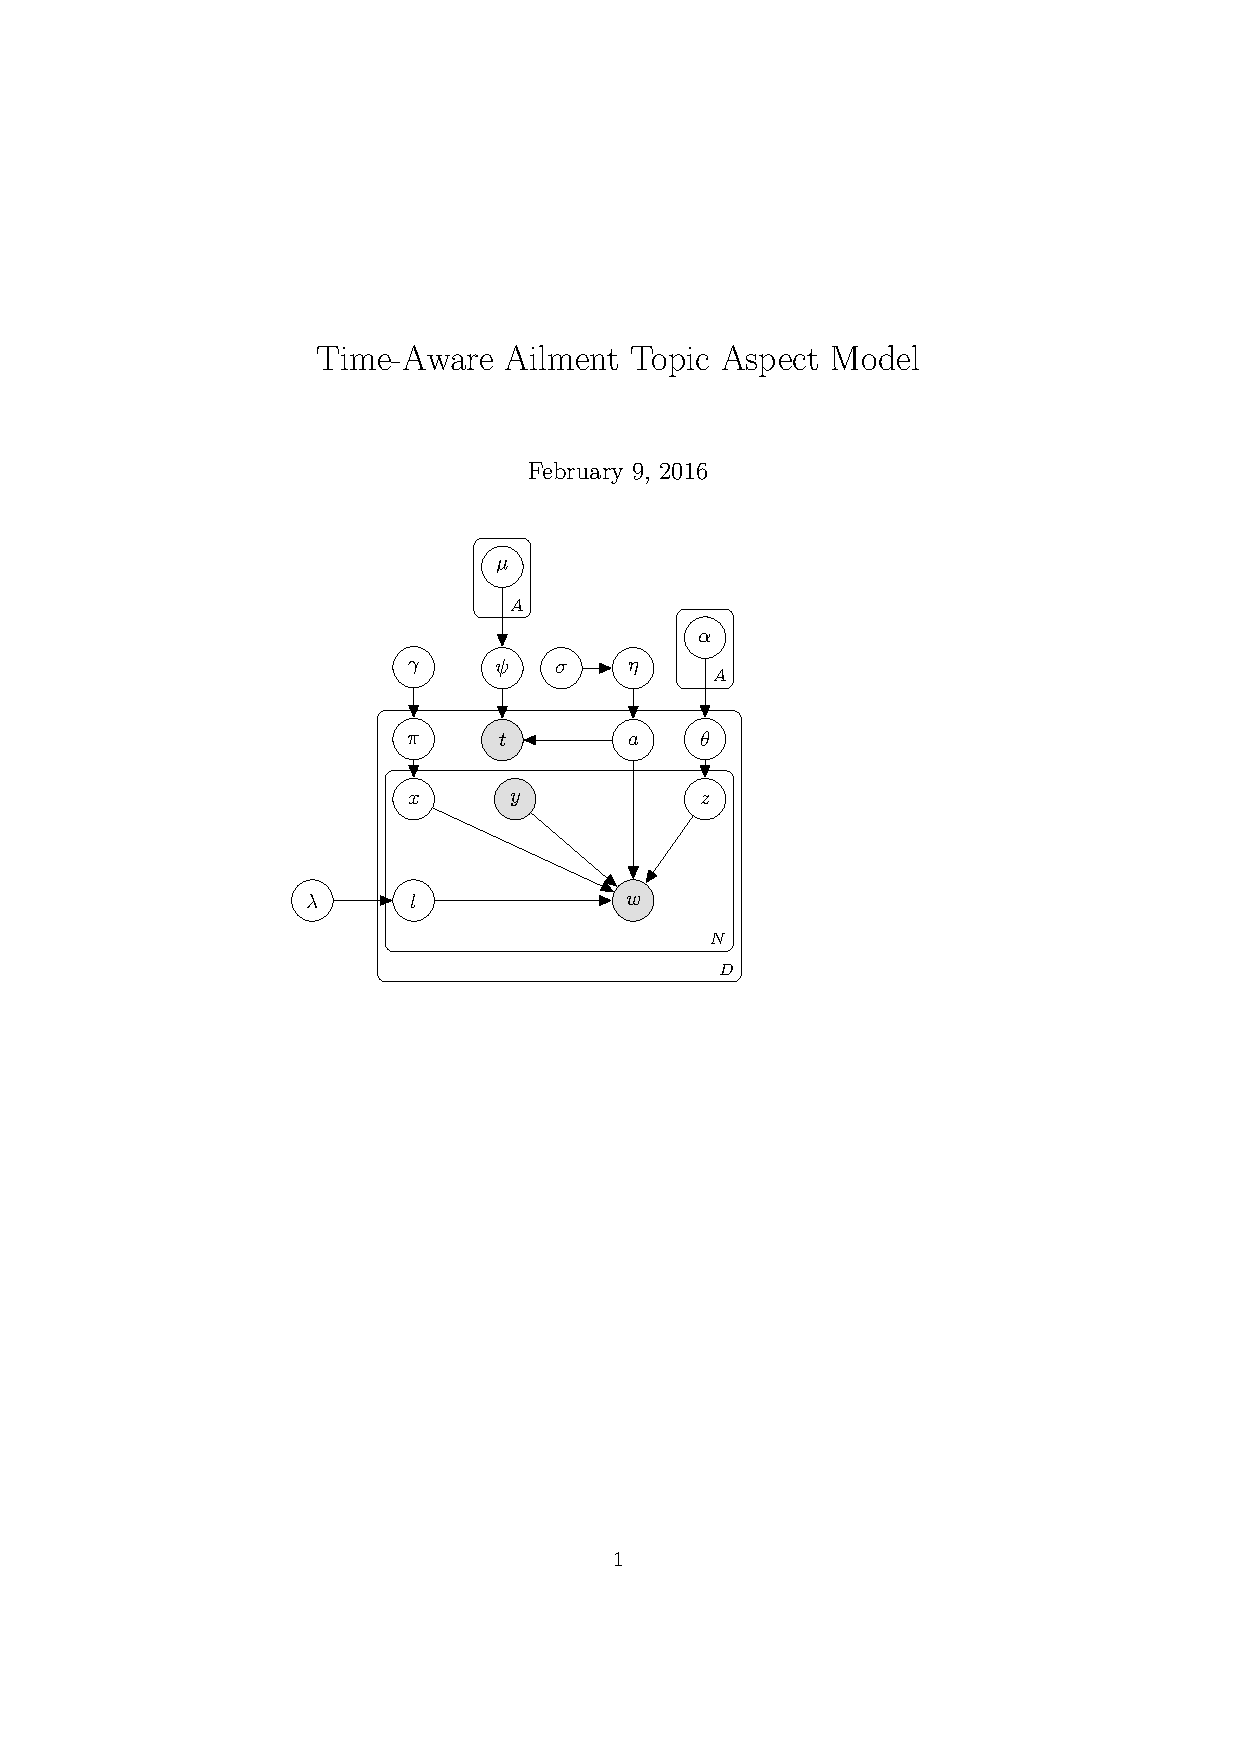
\includegraphics[width=0.45\textwidth]{tikz/plate.pdf}}
%\caption{Time-Aware Ailment Topic Aspect Model.}
%\label{T_atam}
%\end{figure}
\paragraph{Generative Process}
\begin{myEnumerate}
 \item Set the background switching binomial $\lambda$
 \item Draw an ailment distribution $\eta \sim Dir(\sigma)$ 
 \item Draw A multinomials $\psi_A \sim Dir(\mu)$
 \item Draw word multinomials $\phi \sim Dir(\beta)$ for the topic, ailment, and background distributions
 \item For each message $1\ \leq m\leq D$
 \begin{myEnumerate}
  \item Draw a switching distribution $\pi \sim Beta(\gamma_0,\gamma_1)$
  \item Draw an ailment $a\sim Mult(\eta)$
  \item Draw a time stamp $t \sim Mult(\psi_a)$
  \item Draw a topic distribution $\theta \sim Dir(\alpha_a)$
  \item For each word $w_i\in N_m$
  \begin{myEnumerate}
   \item Draw aspect $y_i\in\{0,1,2\}$(observed)
   \item Draw background switcher $l\in\{0,1\}\sim Bi(\lambda)$
   \item if l == 0:
   \begin{myEnumerate}
    \item Draw $w_i\sim Mult(\phi_{B,y})$(a background)
   \end{myEnumerate}
   \item Else:
   \begin{myEnumerate}
    \item Draw $x_i\in \{0,1\} \sim Bi(\pi)$
    \item If $x_i == 0:$(Draw word from topic z)
    \begin{myEnumerate}
     \item Draw topic $z_i\sim Mult(\theta)$
     \item Draw $w_i \sim Mult(\phi_z)$
    \end{myEnumerate}
    \item Else:(draw word from ailment a aspect y)
    \begin{myEnumerate}
     \item Draw $w_i \sim Mult(\phi_{a,y})$
    \end{myEnumerate}
    
        \end{myEnumerate}

   \end{myEnumerate}
   


  \end{myEnumerate}


\end{myEnumerate}
